\documentclass[convert={density=600,outext=.png}]{standalone}
\usepackage{tikz}
\usetikzlibrary{bayesnet}

\begin{document}

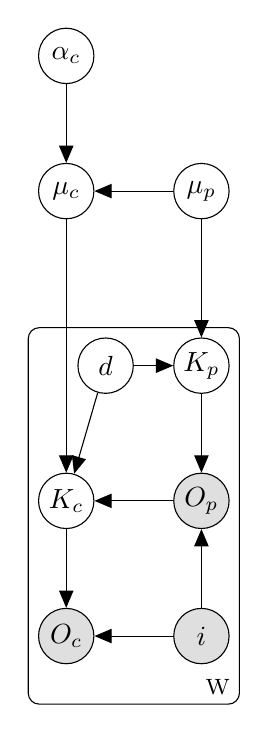
\begin{tikzpicture}[x=1cm,y=1cm]
  
   % Nodes
  \node[latent, ] (mu_p) {$\mu_{p}$};
  \node[latent, left = of mu_p] (mu_c) {$\mu_{c}$};

  \node[latent, above = of mu_c] (alpha_c) {$\alpha_{c}$};

  \node[latent, below = 1.5 of mu_p] (K_p) {$K_{p}$};
  \node[obs, below = of K_p] (O_p) {$O_{p}$};

  \node[latent, left =  of O_p] (K_c) {$K_{c}$};
  \node[obs, below = of K_c] (O_c) {$O_{c}$};

  \node[latent, left = .5 of K_p] (d) {$d$};

  \node[obs, right =  of O_c] (i) {$i$};

  % Edges
  \edge{mu_p}{mu_c};

  \edge{d}{K_c}

  \edge{d}{K_p}

  \edge{mu_c}{K_c};
  \edge{K_c}{O_c};

  \edge{mu_p}{K_p};
  \edge{K_p}{O_p};

  \edge{alpha_c}{mu_c}

  \edge{O_p}{K_c}

  \edge{i}{O_c}
  \edge{i}{O_p}

  % Plates
  \plate {plate_w} {(K_c)(O_c)(d)(K_p)(O_p)} {W};  
\end{tikzpicture}

\end{document}